\documentclass{beamer}
\usepackage[utf8]{inputenc}
\usepackage{graphicx}
\usepackage{listings}

\usepackage{xcolor}

\lstdefinestyle{base}{
	language=C++,
	emptylines=1,
	breaklines=true,
	basicstyle=\ttfamily\color{black},
	moredelim=**[is][\bf\color{red}]{@}{@},
}

\usetheme[]{boxes}
\usecolortheme{seagull}
%\usepackage{french}
\title{Modèles et techniques en programmation parallèle hybride et multi-c\oe urs}
\subtitle{Quelques notions d'optimisation séquentielle}
\author{Marc Tajchman}\institute{CEA - DEN/DM2S/STMF/LMES}
\date{10/08/2020}
\begin{document}

\begin{frame}
\titlepage
\end{frame}

\large
\begin{frame}
	Deux ``règles d'or'' :
	\begin{itemize}
		\item Avant/après optimisation, avant/après parallélisation, il faut s'assurer que le code sur lequel on travaille, donne des résultats corrects.
		
		\item Avant de paralléliser un code et/ou avant d'optimiser le parallélisme, il faut optimiser la partie séquentielle d'un code.
	\end{itemize}
\end{frame}

\begin{frame}
	Pour évaluer l'optimisation d'un code, on utilise des outils de mesure de performance.
	Il existe de nombreux moyens de mesurer le temps d’exécution de code ou de parties de
	code :
	
        \medskip
	\begin{itemize}
		\item \textcolor{blue}{Commande unix {\tt time}} : mesure globale (temps ressenti par l’utilisateur)
        \medskip

        \item \textcolor{blue}{Fonctions définies par le langage de programmation} et utilisables depuis l’intérieur du code :
	        \begin{itemize}
	          	\item {\tt second(...)} (fortran),
	          	\item {\tt gettimeofday(...)} (C/C++),
	          	\item {\tt std::clock()} (C++),
	          	\item {\tt time.time()} (python)
	          	\item {\tt 	tic/toc} (matlab),
	          	\item ...
          	\end{itemize}
		Permet de mesurer le temps d’exécution d’un groupe d’instructions.
		
		\textcolor{blue}{Penser à vérifier dans la documentation quelle est la précision des mesures.}
	\end{itemize}

\end{frame}

\begin{frame}
	\begin{itemize}
	\item \textcolor{blue}{Librairies}, par exemple MPI, OpenMP, PAPI
	
	On ajoute dans le code des appels à des fonctions de la librairie.

	\medskip
	\begin{itemize}
	\item MPI et OpenMP proposent des fonctions pour mesurer le temps de calcul :	{\tt MPI\_Wtime(), omp\_get\_wtime()}.
	\medskip
	
	\item PAPI 
	
	\hbox{\small(\url{https://icl.cs.utk.edu/projects/papi/wiki/Main_Page})}
	\medskip
	
	est une librairie qui donne des informations très précises.
	
	\medskip
	 Permet de consulter des compteurs système très bas niveau (par exemple : nombre
	 d’opérations, utilisation des caches, registres, etc.)
	\end{itemize}
	\end{itemize}

	
\end{frame}

\begin{frame}
	\begin{itemize}
	\item  \textcolor{blue}{Outils externes de ``profilage''}
	
	\medskip
	Ajoutent automatiquement des points de mesure dans le
	code (gprof), s’interposent entre le code et le système pour récupérer des informations
	(valgrind, perf,
vtune (intel), etc.)
		
	\medskip
	Permet de connaître des informations intermédiaires : nombre d’appels et temps
	moyen d’exécution de fonctions par exemple (gprof, valgrind).
	
	Certains sont plus précis et descendent au niveau de l'instruction (perf, vtune)
	\end{itemize}

\vfill
	Les outils de mesure perturbent les temps de calcul et, en général, il faut les utiliser avec
	une version ``debug''. Ils donnent seulement une indication sur les endroits du code les plus
	intéressants à optimiser. De toute façon, à la fin, il faut mesurer les temps calculs sur la
	version ``release'' (on a parfois des surprises) .
\end{frame}

\begin{frame}
\section{Programmation s\'equentielle efficace}
\frametitle{Programmation s\'equentielle efficace}

\bf
\textcolor{blue}{Pour obtenir un code efficace (en temps d'ex\'ecution), il faut:}

\begin{itemize}
	\item utiliser les algorithmes les plus efficaces possible (pas couvert par ce cours)
	
	\item organiser le placement des donn\'ees (am\'eliorer la localit\'e spatiale)
	
	\item organiser la s\'equence d'instructions (am\'eliorer la localit\'e temporelle)

	\item \'ecrire les instructions pour qu'elles soient les plus rapides possibles (éviter de calculer plusieurs fois la même expression, \'eviter si possible les tests, ``faciliter le travail du compilateur'')
\end{itemize}
\end{frame}

\begin{frame}[fragile]
	Une bonne utilisation de la mémoire est très importante pour l'optimisation de code.
	\bigskip

	Exemple : si \verb|u| et \verb|v| sont des vecteurs de taille \verb|n > 4|, on veut calculer la boucle :

\begin{equation}
\begin{array}{l}
for (i=1; i<n-1; i++) \\
\quad  v_i = (u_{i-1} + 2*u_{i} + u_{i+1})/4;
\end{array}
\end{equation}

\end{frame}

\begin{frame}
	Supposons un système idéalisé par: 
	\begin{itemize}
		\item un processeur, 
		\item une mémoire cache de taille 8 (4 lignes cache de taille 2),
		\item la mémoire centrale
	\end{itemize}
	\begin{center}
	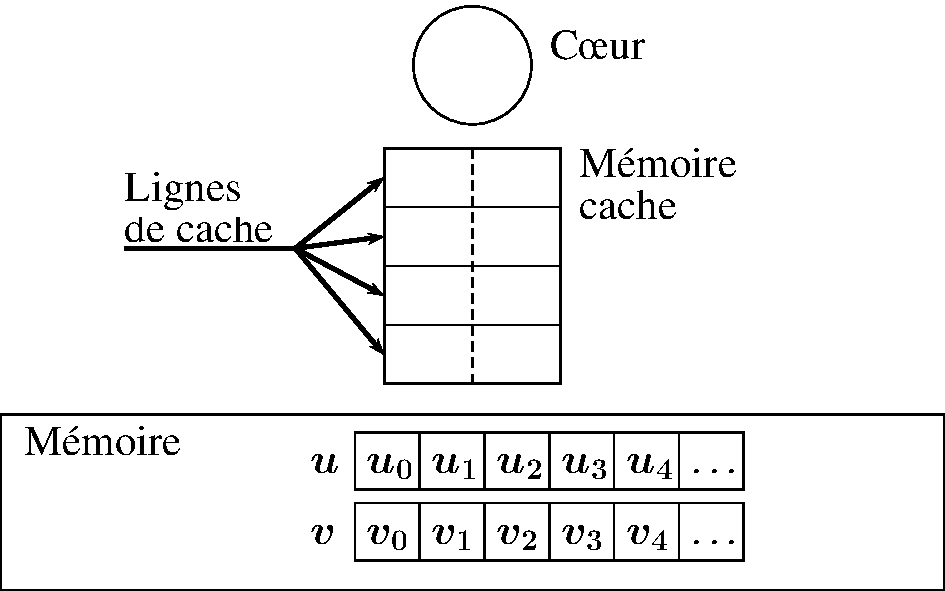
\includegraphics[scale=0.5]{../../Images/sequentiel}
   \end{center}
\end{frame}

\begin{frame}
	\parbox[t][1cm]{10cm}{1. Avant d'exécuter $v_1 = (u_0 + 2*u_1 + u_2)/4$ :}
	\begin{center}
		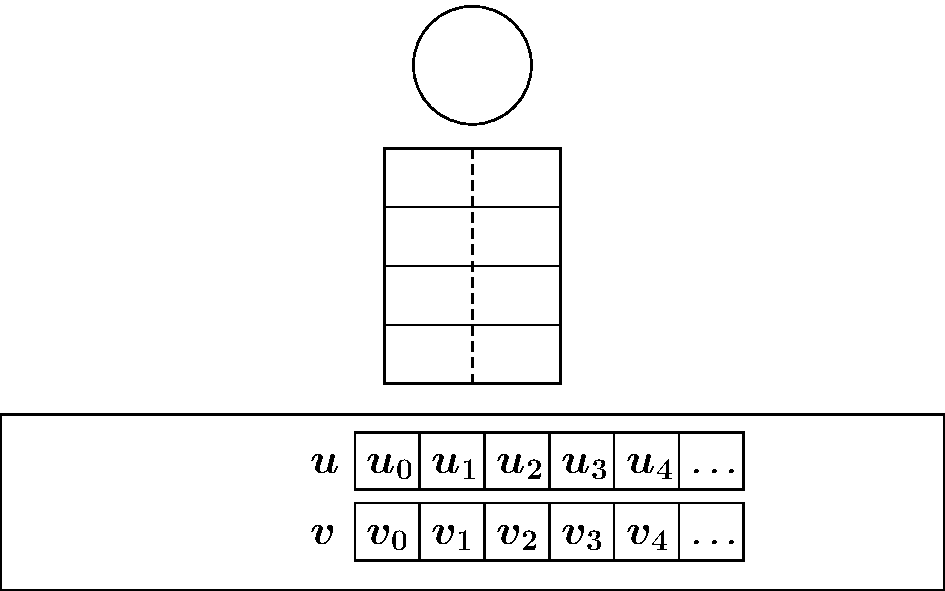
\includegraphics[scale=0.6]{../../Images/sequentiel0}
	\end{center}
\end{frame}
\begin{frame}
	\parbox[t][1cm]{10cm}{2. Les blocs contenant $u_0$, $u_1$, $u_2$ et $v_1$ (3 blocs) sont copiés dans la mémoire cache :}
	\begin{center}
		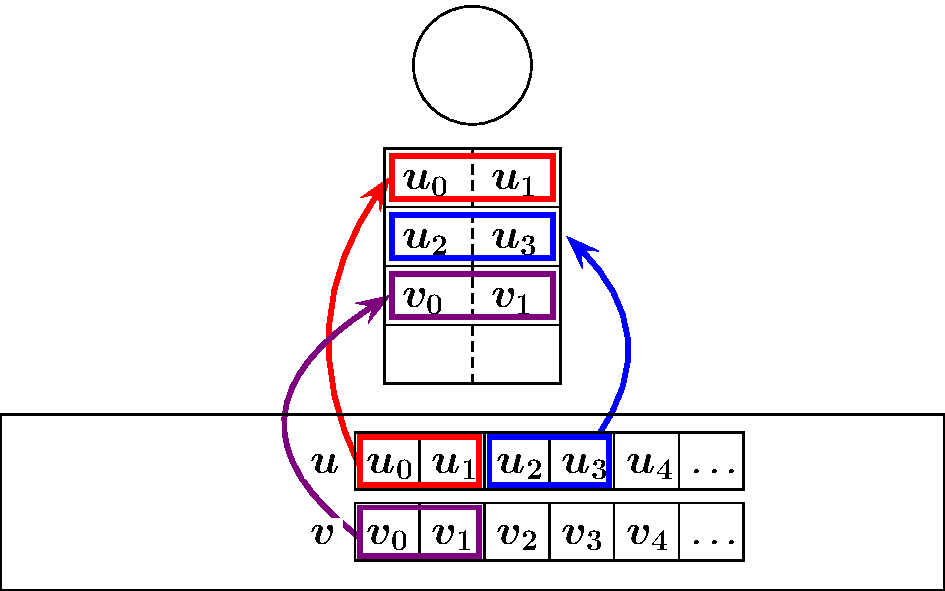
\includegraphics[scale=0.6]{../../Images/sequentiel1}
	\end{center}
\end{frame}
\begin{frame}
	\parbox[t][1cm]{10cm}{3. Le c\oe ur utilise les copies de $u_0$, $u_1$, $u_2$ de la mémoire cache, calcule l'expression et place le résultat dans la mémoire cache :}
	\begin{center}
		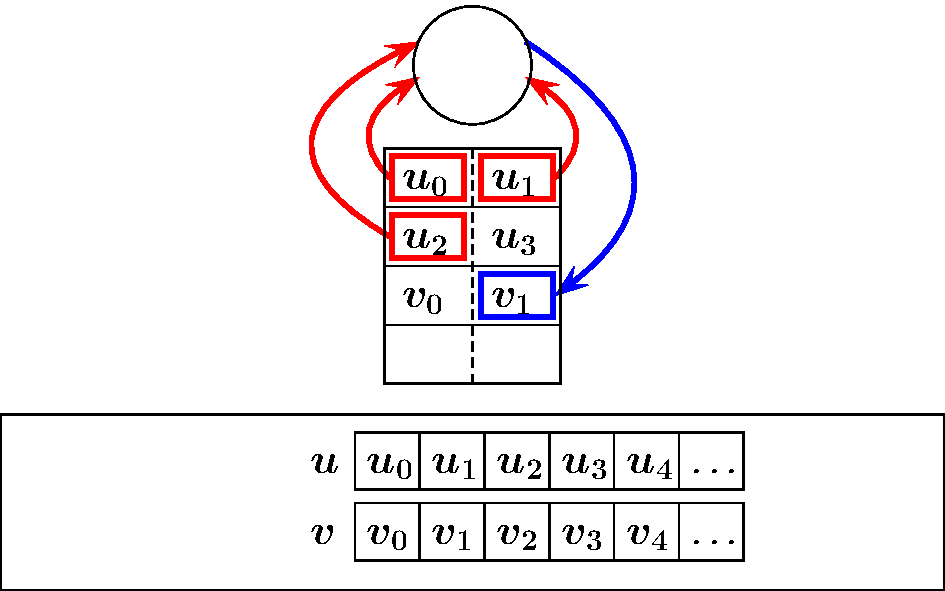
\includegraphics[scale=0.6]{../../Images/sequentiel2}
	\end{center}
\end{frame}
\begin{frame}
	\parbox[t][1cm]{10cm}{4. Le bloc contenant le résultat est recopié dans la mémoire principale :}
	\begin{center}
		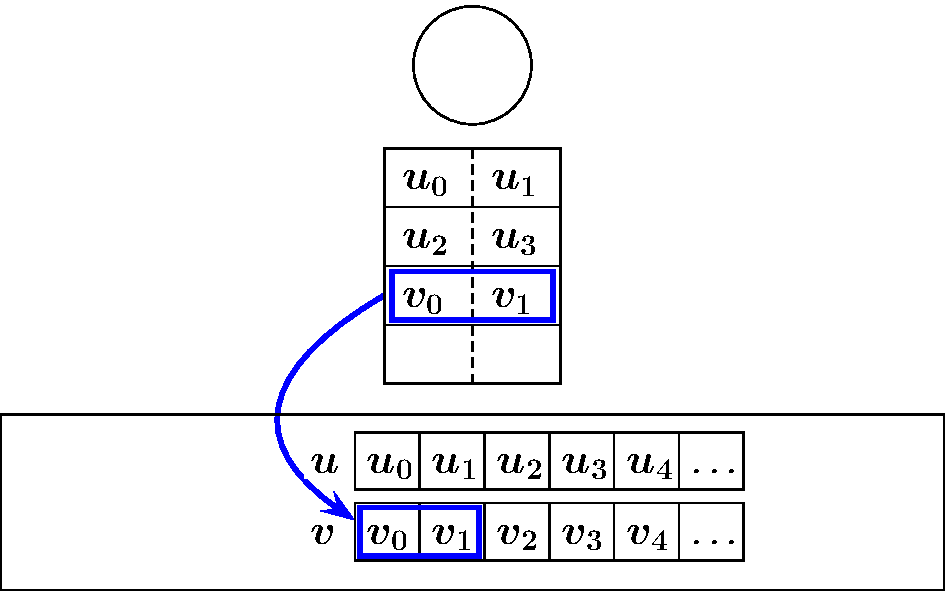
\includegraphics[scale=0.6]{../../Images/sequentiel3}
	\end{center}
\end{frame}
\begin{frame}
	\parbox[t][1cm]{10cm}{5. Le calcul de l'instruction suivante $v_2 = (u_1 + 2*u_2 + u_3)/4$ peut commencer:}
	\begin{center}
		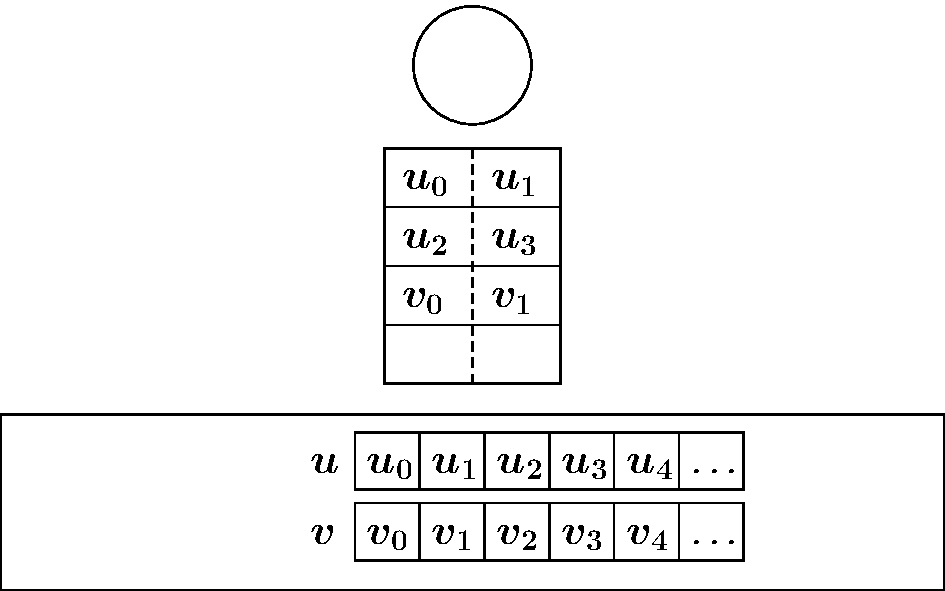
\includegraphics[scale=0.6]{../../Images/sequentiel4}
	\end{center}
\end{frame}
\begin{frame}
	\parbox[t][1cm]{10cm}{6. Les composantes de $u$ nécessaires \textcolor{red}{sont déjà dans la mémoire cache}, seul le bloc contenant la composante $v_2$ doit être copié dans la mémoire cache :}
	\begin{center}
		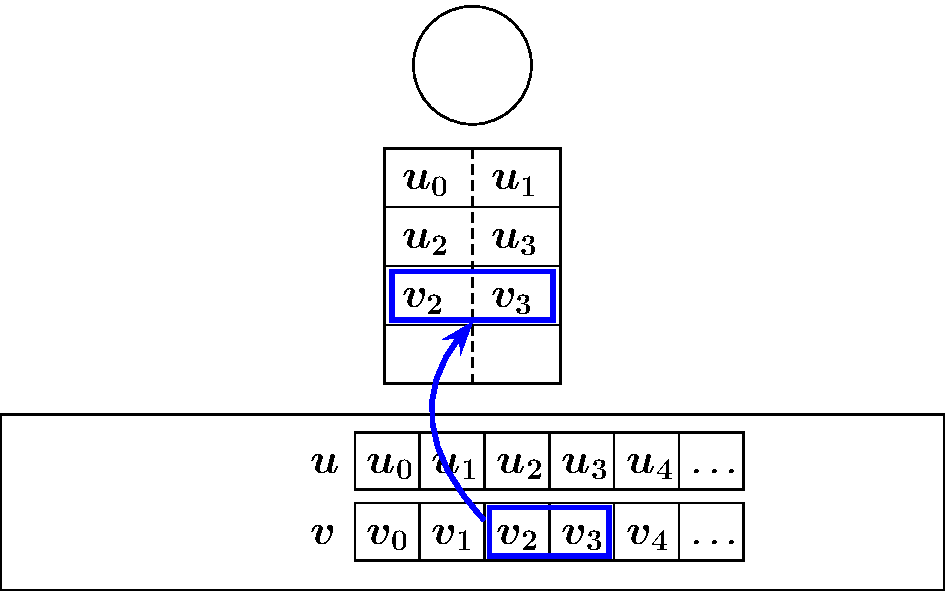
\includegraphics[scale=0.6]{../../Images/sequentiel5}
	\end{center}
\end{frame}
\begin{frame}
	\parbox[t][1cm]{10cm}{6. Le c\oe ur utilise les copies de $u_1$, $u_2$, $u_3$ de la mémoire cache, calcule l'expression et place le résultat dans la mémoire cache :}
	\begin{center}
		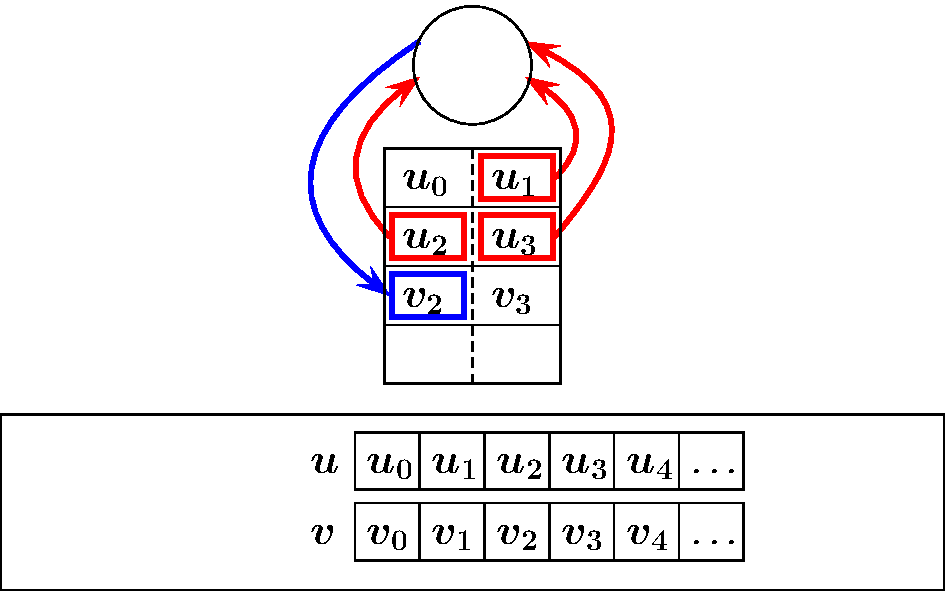
\includegraphics[scale=0.6]{../../Images/sequentiel6}
	\end{center}
\end{frame}
\begin{frame}
	\parbox[t][1cm]{10cm}{6. Le bloc contenant le résultat est recopié dans la mémoire principale :}
	\begin{center}
		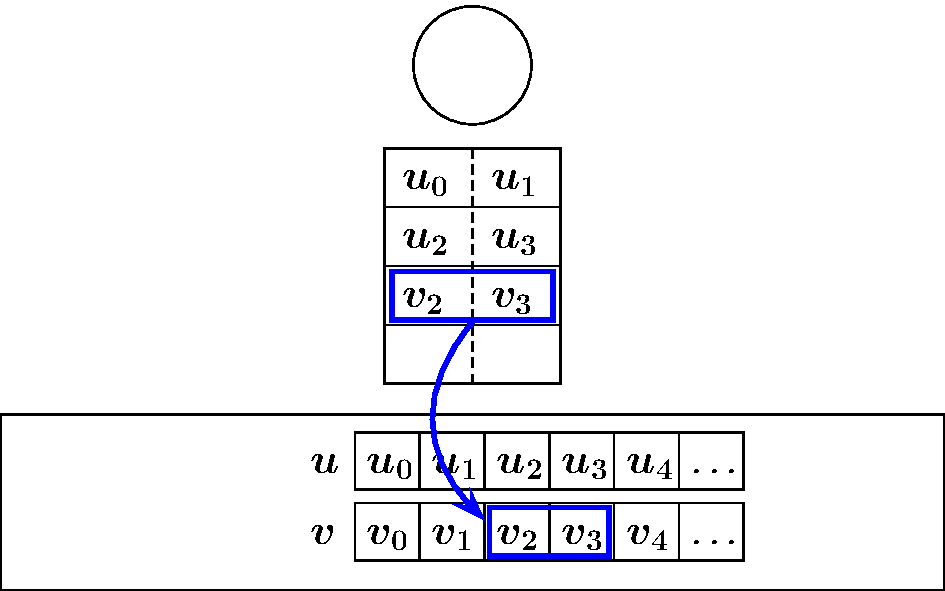
\includegraphics[scale=0.6]{../../Images/sequentiel7}
	\end{center}
\end{frame}

\begin{frame}
	En résumé :
	\begin{itemize}
		\item La première instruction $v_1 = (u_0 + 2*u_1 + u_2)/4$ utilise
		\begin{itemize}
			\item 4 transferts (lents) mémoire principale - mémoire cache
			\item 4 transferts (rapides)  mémoire cache - c\oe ur
		\end{itemize} 
	\smallskip
		\item La deuxième instruction $v_2 = (u_1 + 2*u_2 + u_3)/4$ utilise
		\begin{itemize}
			\item 2 transferts (lents) mémoire principale - mémoire cache
			\item 4 transferts (rapides) mémoire cache - c\oe ur
		\end{itemize}
	\end{itemize}
\vfill
    Examiner et tester l'exemple {\it Exemple1} 
    
\vfill
    Sans mémoire cache, toutes les itérations prendraient (à peu près) le même temps.
    
    La mémoire cache améliore beaucoup le temps de calcul de presque toutes les itérations 
    
    \begin{quote}
    	\textcolor{blue}{Attention, la configuration matérielle sera différente du cas idéalisé ci-dessus, mais on devrait voir la différence entre la première itération et les suivantes.}
    \end{quote}

\end{frame}

\begin{frame}
	\begin{center}
	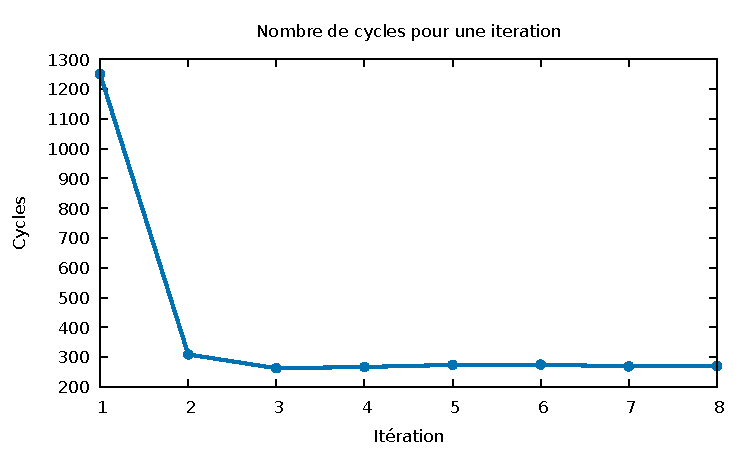
\includegraphics[scale=0.8]{Exemples/Exemple1/cycles.pdf}
	\end{center}

Un cycle est l'unité de temps pour le processeur. Le processeur qui a été utilisé ici, a une fréquence de 3 GHz.
Un cycle prend à peu près $0.3\ 10^{-9}$ secondes. 
\vfill

Sur le graphique, une itération (sauf la première) prend $0.6\ 10^{-7}$ secondes.
\end{frame}

\begin{frame}
\vfill
On voit donc qu'il est important de bien utiliser la mémoire cache.

\vfill
   \textcolor{blue}{Deux règles sont déduites de ce comportement : optimiser les localités spatiale et temporelle.}
\vfill 
\end{frame}

\begin{frame}
\frametitle{Localit\'e spatiale}
Règle:  \textcolor{red}{autant que possible, utiliser des zones m\'emoires proches les unes des autres dans une s\'equence d'instructions}
	\vfill
\begin{quote}
	Le transfert entre m\'emoire centrale et m\'emoire cache se fait par bloc de donn\'ees.
	
	Donc, si une donn\'ee est \`a c\^ot\'e d'une donn\'ee qui vient d'\^etre utilis\'ee (et donc transf\'er\'ee en m\'emoire cache), un nouveau transfert sera peut-\^etre inutile.
\end{quote}

\vfill
Voir l'\textcolor{blue}{Exemple2}
\end{frame}

\begin{frame}
\frametitle{Localit\'e temporelle}
Règle: 
	\textcolor{red}{autant que possible, pour une zone m\'emoire, les instructions qui l'utilisent doivent s'ex\'ecuter de façon rapproch\'ee dans le temps}
	\vfill
	
	\begin{quote}
		La m\'emoire cache \'etant de petite taille, le gestionnaire m\'emoire, s'il a besoin de place, effacera dans la m\'emoire cache les donn\'ees les plus anciennes.
		
		Si une donn\'ee est utilis\'ee par plusieurs instructions proches dans le temps, elle sera maintenue plus longtemps en m\'e\-moi\-re cache (et donc n\'ecessitera moins de transferts)
	\end{quote}

\vfill
Voir l'\textcolor{blue}{Exemple3}
\end{frame}

\begin{frame}[fragile]
\frametitle{Utilisation du // interne au processeur}
Règles: 
\begin{itemize}
	\item essayer de rassembler plusieurs instructions simples en une seule (quand cela a un sens),
	\begin{quote}
		utiliser au maximum la pr\'esence de plusieurs unit\'es de calcul (additionneurs, multiplicateurs, etc) dans un c\oe ur
	\end{quote}
	\item  essayer d'\'eviter les tests
	\begin{quote}
		simplifier le travail du processeur (encha\^{i}nement des instructions le plus d\'eterministe possible).
	\end{quote}
\end{itemize}


\end{frame}

\begin{frame}[fragile]
Exemple: remplacer
\begin{lstlisting}
for (i=0; i<n; i++) {
  u[i] = u0[i];
  if (terme1) u[i] += a*v[i];
  if (terme2) u[i] += b*w[i];
}
\end{lstlisting}

par:
\begin{lstlisting}
if (terme1) aa = a; else aa = 0.0;
if (terme2) bb = b; else bb = 0.0;
for (i=0; i<n; i++) {
   u[i] = u0[i] + aa*v[i] + bb*w[i];
}
\end{lstlisting}

\end{frame}

\end{document}
